\cotefile{43}
\scanpage{145}
\mspage{3}
% archive sheet number: 144
of $k$ at $P$. $\prod$ denotes direct product (compact), $\coprod$ denotes direct sum (discrete), and $\unsure{\underline{\prod}|\prod'}$ denotes restricted direct product, relative to the subgroups $H^1(A_P,\widetilde M)$, (locally compact). The three groups $H^i$ are viewed as discrete and accordingly the $\widehat{H^i}$ are compact. The maps $\alpha_i$ are induced by the canonical maps $G_{k_P}\longrightarrow G_A$. The maps $\beta_i$ are defined by $\beta_i(\widetilde M)=\widehat{\alpha_{2-i}(M)}$. The map $\gamma$ will be explained below when we discuss proofs; its image is finite in all cases. We have $\delta(\widetilde M)=\deleted{\unsure{\delta}}\widehat{\gamma(M)}$. If we take the pontrjagin dual of the sequence for $M$ we get the sequence for $\widetilde M$.

\uline{Corollary 1}: \uline{If} $S$ \uline{is finite, then} $H^r(A,M)$ \uline{is finite for all} $r$. \uline{If in this case we define}
\[
\chi(A,M)=\frac{\operatorname{Card}H^0(A,M)\;\operatorname{Card}H^2(A,M)}{\operatorname{Card}H^1(A,M)}
\]
\uline{then} $\chi(A,M)$ \uline{is ``multiplicative'' in} $M$ \uuline{except} \uline{in case} $k$ \uline{is real and} $m$ \uline{is even. In all cases we have}
\[
\frac{\chi(A,M)\,\chi(A,\widetilde M)}{\operatorname{Card}H^3(A,M)}=
\begin{cases}
1, & \text{\uline{in case} $(F)$}\\
m^{-[k:\unsure{Q|\mathbb Q}]}, & \text{\uline{in case} $(N)$}.
\end{cases}
\]

\uline{Corollary 2}: \uline{The kernel of} $H^2(A,M)\xrightarrow{\alpha_2(M)}\coprod_{P\in S}H^2(k_P,M)$ \uline{is finite and is canonically dual to the kernel of} $H^1(A,\widetilde M)\xrightarrow{\alpha_1(\widetilde M)}\underline{\prod}_{P\in S}H^1(k_P,\widetilde M)$.

Notice that the kernel of $\alpha_1(M)$ is completely constructible in finite terms, as follows. Let $A'$ be an unramified finite extension of $A$ such that $M$ is really a $G_{A'/A}$-module. Let $A''$ be the maximal abelian unramified extension of $A'$ such that all primes $P'$ of $k'$ lying over $P$ in $S$ split completely in $k''$. (Note that $A''=A'$ if $\unsure{\mathbb P|P|\mathscr P}(A')=0$, especially if $S=\text{all primes}$) Let $G=G_{A''/A}$ and let $(G_i)$, $1\leq i\leq h$, denote the subgroups of $G$ which occur as decomposition groups (for $k''/k$) of primes $P\in S$. Then we have

\uline{Proposition \deleted{\unsure{3.1}} 3.2}: \uline{Notations being as above, the kernel of} $\alpha_1(M):H^1(A,M)\longrightarrow\underline{\prod}H^1(k_P,M)$ \uline{is the isomorphic image, under inflation, of the kernel of}
\[
H^1(G,M)\xrightarrow{(\operatorname{res}_{G_i}^{G})_{1\leq i\leq h}}\prod_{i=1}^{h}H^1(G_i,M).
\]

\uline{Corollary 1}: $\operatorname{Ker}\alpha_1(M)$ \uline{is annihilated by the ratio of the global degree} $[k'':k]$ \uline{by the least common multiple of the local degrees for primes} $P$ \uline{in} $S$ \uline{in} $k''/k$. \uline{In particular}, $\alpha_1^{(M)}$ \uline{is injective if} $M$ \uline{is a} $G_{A'/A}$-\uline{module when} $A'/A$ \uline{is cyclic and the class number of} $A'$ \uline{is prime to} $m$.

\scanpage{146}
% archive sheet number: 145
\diagram{\fbox{\begin{tikzcd}[ampersand replacement=\&,column sep=small,row sep=large]
0\arrow[r] \& \unsure{\underline{\prod}|\coprod}_{p\in S}\widehat{H^2(k_p,\widetilde M)}\arrow[r] \& \widehat{H^2(\unsure{O|\mathcal O},\widetilde M)}\arrow[r,"{\inserted{\unsure{\overline{H^0(O,M)}|H^0(O,M)}}}"] \& \prod_{P\in S}\unsure{\widehat H^0|\widetilde H^0}(k_p,M)\arrow[r] \& \widehat{H^1(O,\widetilde M)}\\
{}\arrow[r] \& H^1(O,M)\arrow[r] \& \underline{\prod}_{p\in S}H^1(k_p,M)\arrow[r] \& \widehat{H^0(O,\widetilde M)}. \& {}\\
{}\arrow[r] \& H^2(O,M)\arrow[r] \& \underline{\prod}_{p\in S}H^2(k_p,M)\arrow[r] \& 0 \& {}
\end{tikzcd}}}

\diagram{\fbox{\begin{tikzcd}[ampersand replacement=\&]
H^r(O,M)\arrow[r,"\sim"] \& \underline{\prod}_{p\in S}H^r(k_p,M)
\end{tikzcd}}\quad $r>2$}

If
\[
\unsure{\vcenter{\hbox{\begin{tikzpicture}[x=.6ex,y=1ex]\draw (0,1)--(0,0)--(2,0)--(2,1);\draw (1,0)--(1,1);\end{tikzpicture}}}|\mathrm{III}}(O,M)=\operatorname{Ker}\bigl(H^1(O,M)\longrightarrow\underline{\prod}_{p\in S}H^1(k_p,M)\bigr)
\]
is finite

$M$ \unsure{var\textsuperscript{té}|variété|vaut|varie} \unsure{abélienne|définie} \unsure{sur} un corps de \unsure{nombres} ---

\scanpage{147}
% archive sheet number: 146
Groupes de Galois comme groupes analytiques sur $\mathbb Q_{\unsure{\ell|p}}$, d'après Serre

\scanpage{148}
% archive sheet number: 147
\uline{\unsure{Modules|Module} $\ell$-adiques sur} $S$.

Soit $S$ un préschéma, $\ell$ nb premier, \deleted{\unsure{un}} \deleted{\unsure{Ind} \illegible{1}} $\unsure{\mathscr G|\mathcal G}(S)$ la catégorie des schémas en groupes \inserted{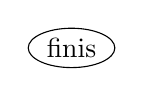
\begin{tikzpicture}[baseline=(n.base)]\node (n) at (0,0) {finis};\draw (0,0) ellipse (.55 and .25);\end{tikzpicture}} étales sur $S$. Un objet de $\operatorname{Ind}(\mathscr G(S))$ est dit ``de type $\mathbb Q_\ell/\mathbb Z_\ell$'' s'il est \uline{strict}, et si ses fibres géométriques sont des \unsure{limites inductives} isomorphes \unsure{à|:} $(\mathbb Q_\ell/\mathbb Z_\ell)^{\unsure{\nu|v}}$ ($\nu$ convenable). Si $S$ est connexe, \deleted{$\xi$ un pt géométrique de $S$, \unsure{alors}} \inserted{$\nu$ est indépendant du} choix du pt géométrique de $S$. Si $\xi$ est un tel pt géométrique, la \deleted{\unsure{anti}} catégorie des \deleted{\unsure{$\mathscr G$}} $G$ ``de type $\mathbb Q_\ell/\mathbb Z_\ell$'' est \deleted{isomorphe} équivalente à la catégorie des \deleted{\unsure{$\xi$}} $\pi_1(S,\xi)$-Modules discrets qui sont isomorphes comme groupes abéliens à $(\mathbb Q_\ell/\mathbb Z_\ell)^\nu$, \deleted{\unsure{donc}} ($\nu$ convenable) i.e. dont le dual au sens de \unsure{Pontrjagin|Pontryagin} [à valeurs dans $\mathbb Q/\mathbb Z$) est \deleted{\unsure{iso}} un module libre de type fini sur $\mathbb Z_\ell^{\deleted{\unsure{\nu|2}}}$.

Par dualité (de Pontrjagin) on obtient les objets de $\operatorname{Pro}\mathscr G(S)$ qui sont ``de type $\mathbb Z_\ell^\nu$''.

Un objet de $\operatorname{Ind}\operatorname{Pro}\mathscr G(S)$ est dit
\scanpage{149}
% archive sheet number: 148
``de type $\mathbb Q_\ell$'' si il est isomorphe \unsure{à|:} un \deleted{\unsure{limite}} système inductif $(G_n)_{n\in\mathbb N}$, où pour tout $n$, on a $G_n=G_0$ $G$ étant ``de type $\deleted{\unsure{\mathbb Q}}\mathbb Z_\ell$'', et $\unsure{\varphi_{nm}|\varphi_{mn}}$ (pour $m\geq n$) étant la multiplication par $\ell^{m-n}$. Si $S$ est connexe, de pt géométrique $\xi$, alors la catégorie \deleted{de} \unsure{ces|des} $G$ est équivalente à la catégorie des espaces vectoriels \inserted{$\unsure{N|V}$} de dim finie sur $\mathbb Q_\ell$, munis d'un hom continu de groupes topologiques $\pi_1(S,\xi)\longrightarrow\deleted{\unsure{\operatorname{GL}(N)}}\operatorname{Aut}(N)$. [Noter que $\pi_1(S,\xi)$ étant compact, il y \unsure{aura|a} un ``réseau'' invariant ...]. Soit de façon générale \inserted{$\unsure{\mathcal V|\mathscr V}_\ell(S)$ la catégorie des objets de $\operatorname{Ind}\operatorname{Pro}\unsure{\mathscr G|\mathcal G}(S)$ qui sont ``de type $\mathbb Q_\ell$'', $\unsure{\mathcal M|\mathscr M}_\ell(S)$ la catégorie des objets} \deleted{\unsure{la catégorie des} \illegible{1}} de $\operatorname{Pro}\mathscr G(S)$ qui sont ``de type $\mathbb Z_\ell$'', alors \deleted{\unsure{on}}
\[
M\unsure{\rightsquigarrow|\longrightarrow|\longmapsto}M\otimes_{\mathbb Z_\ell}\mathbb Q_\ell=(M_n=M,\;M_m\xrightarrow{\ell^{m-n}}M_n)
\]
est un foncteur
\[
\mathcal V_\ell(S)\longrightarrow\mathcal M_\ell(S)
\]
qui est essentiellement surjectif, \inserted{et \uline{fidèle}}, (pas pleinement fidèle en général). Les
\scanpage{150}
% archive sheet number: 149
développements qui suivent ne font intervenir que les $\unsure{\mathcal V|\mathscr V}_\ell(S)$, mais en pratique on partira souvent avec des éléments de $\unsure{\mathcal M|\mathscr M}_\ell(S)$ [ou de façon équivalente par dualité de Pontrjagin, de $\unsure{\mathcal I|\mathrm I}_\ell(S)$].

Soit $S'\longrightarrow S$, il s'en déduit un \inserted{\unsure{diagramme de}} foncteurs \unsure{essentiellement|partiellement} commutatif
\diagram{\begin{tikzcd}[ampersand replacement=\&]
\mathcal I_\ell(S)^\circ\arrow[r,"\sim"]\arrow[d] \& \mathcal M_\ell(S)\arrow[r]\arrow[d] \& \mathcal V_\ell(S)\arrow[d]\\
\mathcal I_\ell(S')^\circ\arrow[r,"\sim"] \& \mathcal M_\ell(S')\arrow[r] \& \mathcal V_\ell(S')
\end{tikzcd}}
les flèches verticales étant des flèches de changement de base. Quand $S$ et $S'$ sont connexes, $\xi'$ un pt géométrique de $S'$, $\xi$ son image dans $S$, d'où
\[
\pi'=\pi_1(S',\xi')\unsure{\text{---}|\longrightarrow}\pi=\pi_1(S,\xi)
\]
alors les foncteurs verticaux s'interprètent [en termes de \deleted{\unsure{$\pi$ et $\pi$}} Modules sur $\pi$ et $\pi'$] par restriction des scalaires

\scanpage{151}
% archive sheet number: 150
Supposons que l'on ait un système projectif $\unsure{\mathscr S|\mathcal S}=(S_i)_{i\in I}$, avec $i_0\in I$ tel que $i\geq i_0$ implique $\varphi_{i_0i}:S_i\unsure{\text{---}|\longrightarrow}S_{i_0}$ est affine. Soit $S=\varprojlim S_i$. Soit $G$ sur $S$, [d'un des trois types envisagés]. Dans beaucoup de situations, on dispose de mieux que d'un groupe sur $S$, mais on dispose \unsure{de l'un|d'un} objet de
\[
\unsure{\mathcal V|\mathscr V}_\ell(\mathscr S)=\underset{\longrightarrow}{\operatorname{Pseudolim}}\mathcal V_\ell(S_i)
\]
[resp. \unsure{en|avec} $\mathcal V_\ell$ remplacé par $\unsure{\mathcal M|\mathscr M}_\ell$, $\unsure{\mathcal I|\mathrm I}_\ell$].

Exemple : Si par exemple, on part d'un \deleted{\unsure{prém}} $S$-schéma abélien \inserted{$A$}, d'où pour $i$ grand un $S_i$-schéma abélien $A_i$, d'où des $T_\ell(A_i)\in\mathcal M_\ell(S_i)$, qui définissent un élément de $\deleted{\unsure{\mathcal V_\ell}}\mathcal M_\ell(\mathscr S)$ [$\ell$ inversible \unsure{en|sur} $S$].
% slanted
\margin{Autre exemple : $X$ schéma \unsure{lisse} et propre sur $S$, $\ell$ premier aux car. rés. de $S$, on prend les faisceaux de Weil $\varprojlim R^if_*(\mathbb Z/\ell^{\unsure{n|u}}\mathbb Z)=R^if_*(\unsure{\mathbb Z_\ell|\mathbb Q_\ell})$ \unsure{mod} torsion\unsure{......}}

Supposons pour simplifier les $S_i$ connexes, donc $S$ connexe, soit $\xi$ un pt
\scanpage{152}
% archive sheet number: 151
géométrique de $S$, $\xi_i$ son image dans $S_i$, donc
\[
\unsure{\pi_1|\pi}=\pi_1(S,\xi)\xrightarrow{\sim}\varprojlim_i\pi_i\unsure{[|;}\qquad \pi_i=\pi_1(S_i,\xi_i).
\]
Donc un élément (disons) de $\unsure{\mathcal V|\mathscr V}_\ell(\unsure{\mathscr S|\mathcal S})$ \deleted{s'identifie \unsure{essentiellement à un}} est défini par un vectoriel $V_{\unsure{\ell|i}}$ sur $\mathbb Q_\ell$ où $\pi_i$ opère ``continûment'', avec le ``proviso'' que pour un $W_j$ analogue sur $\pi_j$, un ``homomorphisme'' de $V$ dans $W$ est un élément de
\[
\varinjlim_{\substack{k\\(k\geq i,j)}}\operatorname{Hom}_{S_k}(V_i\times_{S_i}S_k,\;W_j\times_{\unsure{\varphi_j|S_j}}S_k)
\]

% vertical emphasis line in left margin
\margin{\rule{0.4pt}{6\baselineskip}}
Supposons maintenant que \inserted{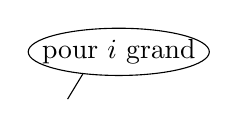
\begin{tikzpicture}[baseline=(n.base)]\node (n) at (0,0) {pour $i$ grand};\draw (0,0) ellipse (1.15 and .3);\draw (-.45,-.27)--(-.65,-.6);\end{tikzpicture}} les \deleted{\unsure{$S_i$}} hom \deleted{$\pi_1(S_j,\unsure{\xi|\xi_j})$} $\pi_j\longrightarrow\pi_i$ aient des images d'indice fini. Cela est le cas si les $S_i$ sont \uline{normaux} \inserted{pour $i$ grand}, et les $\varphi_{ij}:S_j\unsure{\text{---}|\longrightarrow}S_i$ sont dominants et \inserted{définissent des extensions de corps} de type fini.

[on est ramené au cas des \uline{corps}, où on distingue le cas d'une extension \unsure{transcendante}
\scanpage{153}
% archive sheet number: 152
pure ou plus généralement séparable \unsure{primaire}, --- où $\pi_j\unsure{\text{---}|\longrightarrow}\pi_i$ est surjectif --- et d'une extension finie séparable --- où $\pi_j\text{---}\pi_i$ est un isom sur un ss-groupe d'indice fini --- et d'une extension finie radicielle --- où $\pi_j\simeq\pi_i$ --- . Alors les images $G_{\unsure{j|i}}$ des
\[
\pi_{\unsure{j|i}}\longrightarrow\operatorname{Aut}\deleted{\unsure{G}}V_{\unsure{\xi_{i_0}|\xi_i}}
\]
($j\geq i_0$) sont des sous-groupes fermés, \deleted{fermés} d'indice fini les uns dans les autres. Ce système projectif de sous-groupes de $\operatorname{Aut}(V_{i_0})$ \deleted{est défini} a un caractère intrinsèque, est \unsure{remplacé} par un \unsure{cofinal} si on remplace $(S_i)$ par un système cofinal. Par \unsure{Kossul|Koszul}, \uline{ce sont des sous-groupes analytiques $\ell$-adiques} de $\operatorname{Aut}(V_{i_0})$, donc ils ont une algèbre de Lie $\mathfrak g\subset\deleted{\unsure{\mathfrak h|\mathfrak k}}\mathfrak{gl}(V_\xi)=\operatorname{End}_{\mathbb Q_\ell}(V_\xi)$ \uline{indépendante}
\scanpage{154}
% archive sheet number: 153
\uline{de $i$}. \deleted{\unsure{D'où} \illegible{2}} C'est l'\uuline{Algèbre de Serre}

Supposons $S=\operatorname{Spec}(A)$, $A$ anneau \deleted{\unsure{normal}} \deleted{\inserted{intègre}} \deleted{pour fixer les idées}. Alors on a
\[
A=\unsure{\varinjlim_i|\underset{i}{\underline{\lim}}}A_i
\]
les $A_i$ les sous-anneaux de type fini, \deleted{\unsure{normaux sur} $\mathbb Z$.} normaux \inserted{lorsque $A$ l'est} si on y tient.

[N.B. \deleted{Si} Si $A$ contient un corps premier, si ce dernier est de car $p>0$, les $A_i$ sont des algèbres de type fini sur $\mathbb F_p$. Si $A\supset\mathbb Q$, \unsure{on peut aussi envisager} \unsure{ce seul cas|le seul cas|ce seul corps|en cet cas}, et écrire
\[
A=\varinjlim_\alpha B_\alpha
\]
les $B_\alpha$ les (sous-\inserted{$\mathbb Q$}-algèbres de $A$ qui sont de type fini; \deleted{\unsure{Mais généralement}} \inserted{un élément de} $\unsure{\mathcal V|\mathscr V}((A_i))$ en définit un de $\mathcal V((B_\alpha))$, \unsure{mais n'oublions|mais il s'en faut} que les objets \deleted{\unsure{de}} de $\mathcal V((B_\alpha))$, qu'on arrive \unsure{à|:} fabriquer proviennent en fait de $\mathcal V((A_i))$, cf exemples plus haut)\unsure{,|.} On dira
% slanted
\margin{N.B. Pour la formation des \uline{algèbres de Serre}, le \unsure{passage} des $A_i$ aux $B_\alpha$ est sans effet.}
\scanpage{155}
% archive sheet number: 154
qu'on a un \deleted{\unsure{Module}} ``vectoriel $\ell$-adique'' [ou ``Module $\ell$-adique''\unsure{)|]} \uline{attaché \unsure{à|:} $A$} si on a un élément de
\[
\unsure{\mathcal V|\mathscr V}((A_i))=\underset{\longrightarrow}{\operatorname{Pseudolim}}\mathcal V(A_i).
\]
Si $A$ est normal \inserted{(p.ex)} il lui est attaché \deleted{\unsure{une}} \inserted{\unsure{canoniquement}} [pour tt pt géométrique $\xi$ de $S$] une ss-algèbre de Lie $\mathfrak g_\xi$ de $\mathfrak{gl}(V_\xi)$.

D'ailleurs, l'image de $\pi_1(S,\xi)\unsure{\text{---}|\longrightarrow}\operatorname{Aut}(V_\xi)$ définit un autre ss-groupe analytique, donc une algèbre de Lie $\mathfrak g'_\xi\unsure{\ell|l|)}\unsure{\subset|\subseteq}\mathfrak g_\xi$. La formation de $\mathfrak g_\xi$ est \deleted{compatible} \uline{insensible} par \uline{extension \inserted{(dominante)} de la base}, contrairement à celle de $\mathfrak g'_\xi$ [$\mathfrak g'_\xi$ \uline{diminue} quand $(S,\xi)$ est remplacé \unsure{par} $(S',\xi')$ au dessus,].
\margin{\figure{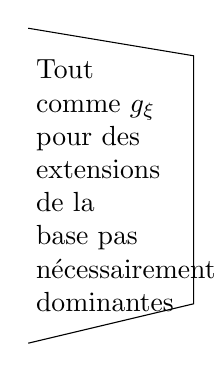
\begin{tikzpicture}\node[align=left,text width=1.9cm,inner sep=0pt] at (0,0) {Tout comme $\mathfrak g_\xi$ pour des extensions de la base pas nécessairement dominantes};\draw (-1.05,2)--(1.05,1.65)--(1.05,-1.5)--(-1.05,-2);\end{tikzpicture}}}
\inserted{Si d'ailleurs $A$ est de type fini \unsure{sur $\mathbb Z$|bien sûr}, on a évidemment $\mathfrak g'_\xi=\mathfrak g_\xi$.}

On constate facilement que [dans le cas général d'un système $(S_i)$ ...] \deleted{\unsure{en faisant}} le choix des \deleted{\unsure{les}} ``\unsure{classes de Chemins|classes de chemins}'' de $\xi$ à $\xi'$ \deleted{\unsure{type}} (\unsure{p\textsuperscript{ce} qu'on a dit|v\textsuperscript{ce} qu'on a dit|vu ce qu'on a dit}) définit
\scanpage{156}
% archive sheet number: 155
un isom $V_\xi\longrightarrow V_{\xi'}$ qui transporte $\mathfrak g_\xi$ en $\mathfrak g_{\xi'}$. \inserted{En particulier, $\mathfrak g_\xi$ est invariant sous le $\pi_1(S_i,\xi)$;} on peut donc définir \unsure{---} un foncteur \inserted{(\unsure{pour les} isomorphismes)} qui \unsure{à|:} tout ``vectoriel de type $\mathbb Q_\ell$ attaché à $(S_i)$'', \inserted{soit $V$,} associe une ``algèbre de Lie de type $\mathbb Q_\ell$ attachée à $(S_i)$'', \deleted{\unsure{disons|d'où un} \illegible{1} ``\unsure{agit}''} $\mathfrak g$, \deleted{qui} [d'où une Ind-Pro-schéma en algèbres de Lie sur $S$ correspondant] \uline{opérant} sur $V$ en un sens évident.

\scanpage{158}
% archive sheet number: 157
\diagram{\begin{tikzcd}[ampersand replacement=\&]
\pi_1(S,\xi)=\varprojlim\pi_1(S_i\unsure{;|,}\xi_i) \arrow[d] \\
G
\end{tikzcd}}
\[\pi_1(S,\xi)\qquad\bullet\]
\figure{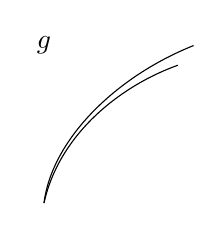
\begin{tikzpicture}
\node at (0,2) {$\mathfrak g$};
\draw (0,0) .. controls (.1,.8) and (.9,1.6) .. (1.9,2);
\draw (0,0) .. controls (.2,.9) and (1,1.5) .. (1.7,1.75);
\end{tikzpicture}}
\diagram{\begin{tikzcd}[ampersand replacement=\&,column sep=large]
\& \overline{k}_0 \arrow[d,no head] \\
\overline{k}_1 \arrow[r,no head] \arrow[d,no head] \& (\overline{k}_1,k_2) \arrow[d,no head] \\
\unsure{K_1|k_1} \arrow[r,no head,"{\text{``\unsure{infini|infinie}''}}"'] \arrow[d,no head] \& k_2 \\
k_1
\end{tikzcd}}
\figure{\begin{tikzpicture}\draw (0,.8)--(.05,.6);\draw (0,.2).. controls (.1,0) .. (.2,-.1);\draw (.5,.8)--(.65,.8);\end{tikzpicture}}
\diagram{\begin{tikzcd}[ampersand replacement=\&]
\& A' \& S \\
\bullet\ A \arrow[ur,no head] \arrow[r] \& A_i
\end{tikzcd}}
\figure{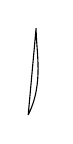
\begin{tikzpicture}\draw (0,0).. controls (.2,.4) and (.1,.8)..(.1,1.1)--(0,0);\end{tikzpicture}}
\[
\begin{aligned}
&\exists\ g\in G\\
&U\ \text{\unsure{voisinage} de }e\\
&(gu)^n\in H\ \text{pour tt }u
\end{aligned}
\]
\diagram{\begin{tikzcd}[ampersand replacement=\&]
A \arrow[r] \& B \\
S \& T \arrow[l] \\
S_i \& T_i \arrow[l] \\
\pi_1(S_i) \& \pi_1(T) \arrow[l]
\end{tikzcd}}
\[\unsure{\mathfrak h_1|\mathfrak g_1}\subset\mathfrak h_2\]
\[
\begin{gathered}
H_1\unsure{\longleftarrow|\deleted{\subset}}\unsure{\widehat\Pi_c|\widehat H_2}\\
H_1\unsure{,\subset|\subset}H_2\\
\cap\\G
\end{gathered}
\]
\diagram{\begin{tikzcd}[ampersand replacement=\&]G\arrow[r,leftrightarrow]\&G'\end{tikzcd}}
\figure{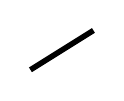
\begin{tikzpicture}\draw[line width=2pt](0,0)--(.8,.5);\end{tikzpicture}}
\diagram{\begin{tikzcd}[ampersand replacement=\&]S\&S'\arrow[l]\end{tikzcd}}
\diagram{\begin{tikzcd}[ampersand replacement=\&]
\&\unsure{\Gamma|\mathscr T}\subset G\times\unsure{C'|G'}\arrow[dl]\arrow[dr]\\
G\&\&C'
\end{tikzcd}}
\diagram{\begin{tikzcd}[ampersand replacement=\&]G\arrow[r]\&C'\end{tikzcd}}
\diagram{\begin{tikzcd}[ampersand replacement=\&,row sep=large]
\begin{gathered}\text{$\unsure{k|\ell}$-groupe de type \unsure{galoisien}}\\\text{avec groupes finis}\end{gathered}\arrow[d,"{\deleted{\unsure{\mathfrak g|F}}}"']\\
\begin{gathered}\text{systèmes projectifs \unsure{stricts}}\\\text{d'algèbres de Lie de}\\\text{dim finie sur }\mathbb Q_\ell\end{gathered}
\end{tikzcd}}
\figure{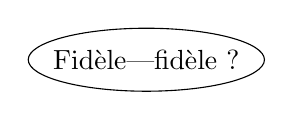
\begin{tikzpicture}\draw (0,0) ellipse (1.5 and .4);\node at (0,0){\unsure{Fidèle|fidèle} \unsure{?}};\end{tikzpicture}}
\uline{Lemme} le th est vrai pour
\[H_1\simeq\mathbb Z_\ell\]
\diagram{\begin{tikzcd}[ampersand replacement=\&,column sep=small,row sep=large]
\begin{gathered}\text{que }H_1\unsure{\subset_{\mathfrak g}|\subset_G|\subset}H_2\\
\text{i.e. }H_1\cap H_2\text{ est}\\\text{ouvert dans }H_1,\\\text{i.e. d'indice fini}\end{gathered}\arrow[r,Rightarrow]
\&\mathfrak h_1\subset\mathfrak h_2\arrow[r,"?"]
\&\begin{gathered}\text{tt \unsure{Germe|groupe}}\\\text{de ss-groupe}\\\text{à un paramètre de}\\H_1\\
\deleted{\unsure{\text{qui a}}\ \unsure{\text{sa}}\ \unsure{H_1}}\ \inserted{\text{est}}\ \text{\unsure{dans|en}}\ H_2\end{gathered}\arrow[d,Rightarrow,"{\deleted{\unsure{H_1}}\ \unsure{\text{cpt}}}"]\\
\&\begin{gathered}\text{par Lemme : si }H\subset G,\text{ et tt élém de }G\text{ a une puiss. en }H,\\\text{alors }H\text{ d'indice fini dans }G.\end{gathered}\arrow[ul,bend left=10,Rightarrow]
\&\begin{gathered}\text{tout}\ \text{élément de }H_1\\\text{a une puissance}\\\text{dans }H_2\end{gathered}
\end{tikzcd}}
\figure{\begin{tikzpicture}\draw (0,0)--(.5,.4);\draw(1.5,1)..controls(2,1.1)and(2,.7)..(2,.3);\draw (3,1) .. controls (4,1) and (3.3,.2)..(5,.2) -- (6.4,.2);\end{tikzpicture}}

\scanpage{159}
% archive sheet number: 158
% margin note written sideways
\margin{$\mathfrak g=(\unsure{\mathfrak g_i|\mathfrak h_i|\mathfrak h'|\mathfrak g'})$}

\scanpage{160}
% archive sheet number: 159
Tableau des $\operatorname{Hom},\underline{\operatorname{Hom}}$\newline
$\operatorname{Ext}^1,\underline{\operatorname{Ext}}^1$\newline
Pour des types simples\newline
de groupes alg. \unsure{comm.}

